\documentclass[12pt,a4paper]{article}
\usepackage{physics}
\usepackage{amssymb}
\usepackage{subcaption}
\usepackage{colortbl}
\usepackage{musicography}
\newcommand{\activity}{Activity 14 -- Logistic regression}
\input{spp.dat}

\begin{document}

\title{\TitleFont \activity}
\author[ ]{\textbf{Kenneth V. Domingo} \\
2015--03116 \\
App Physics 186, 1\textsuperscript{st} Semester, A.Y. 2019--20}
\affil[ ]{\corremail{kvdomingo@up.edu.ph} }

\maketitle
\thispagestyle{titlestyle}

\section*{Results and Discussion}
\setcounter{section}{1}

For this activity \cite{soriano}, I used the banana dataset from \cite{fruits} which has 273 images of bananas separated by underripe, midripe, yellowish-green, and overripe labels.

\subsection{Feature extraction: RGB}
For the training set I decided to take only images of underripe (green) and ripe (yellow) bananas and assign them class numbers 0 and 1, respectively. The feature vector extracted from the images consist only of the mean of each color channel (whose values are normalized to 1), without any further preprocessing or segmentation. I simply reused my code from the previous activity, with minor modifications. The feature space in RGB is shown in Fig. \ref{fig:rgb-features}.

After training all the ripe/unripe images, I then fed in the midripe images and plotted their activations. We can see from Fig. \ref{fig:rgb-preds} that the predictions appear biased toward the upper half, which subjectively does not agree with the corresponding images. Preferably, the predictions are nicely distributed about the center. To this end, I try another approach.

\begin{figure}[htb]
	\centering
	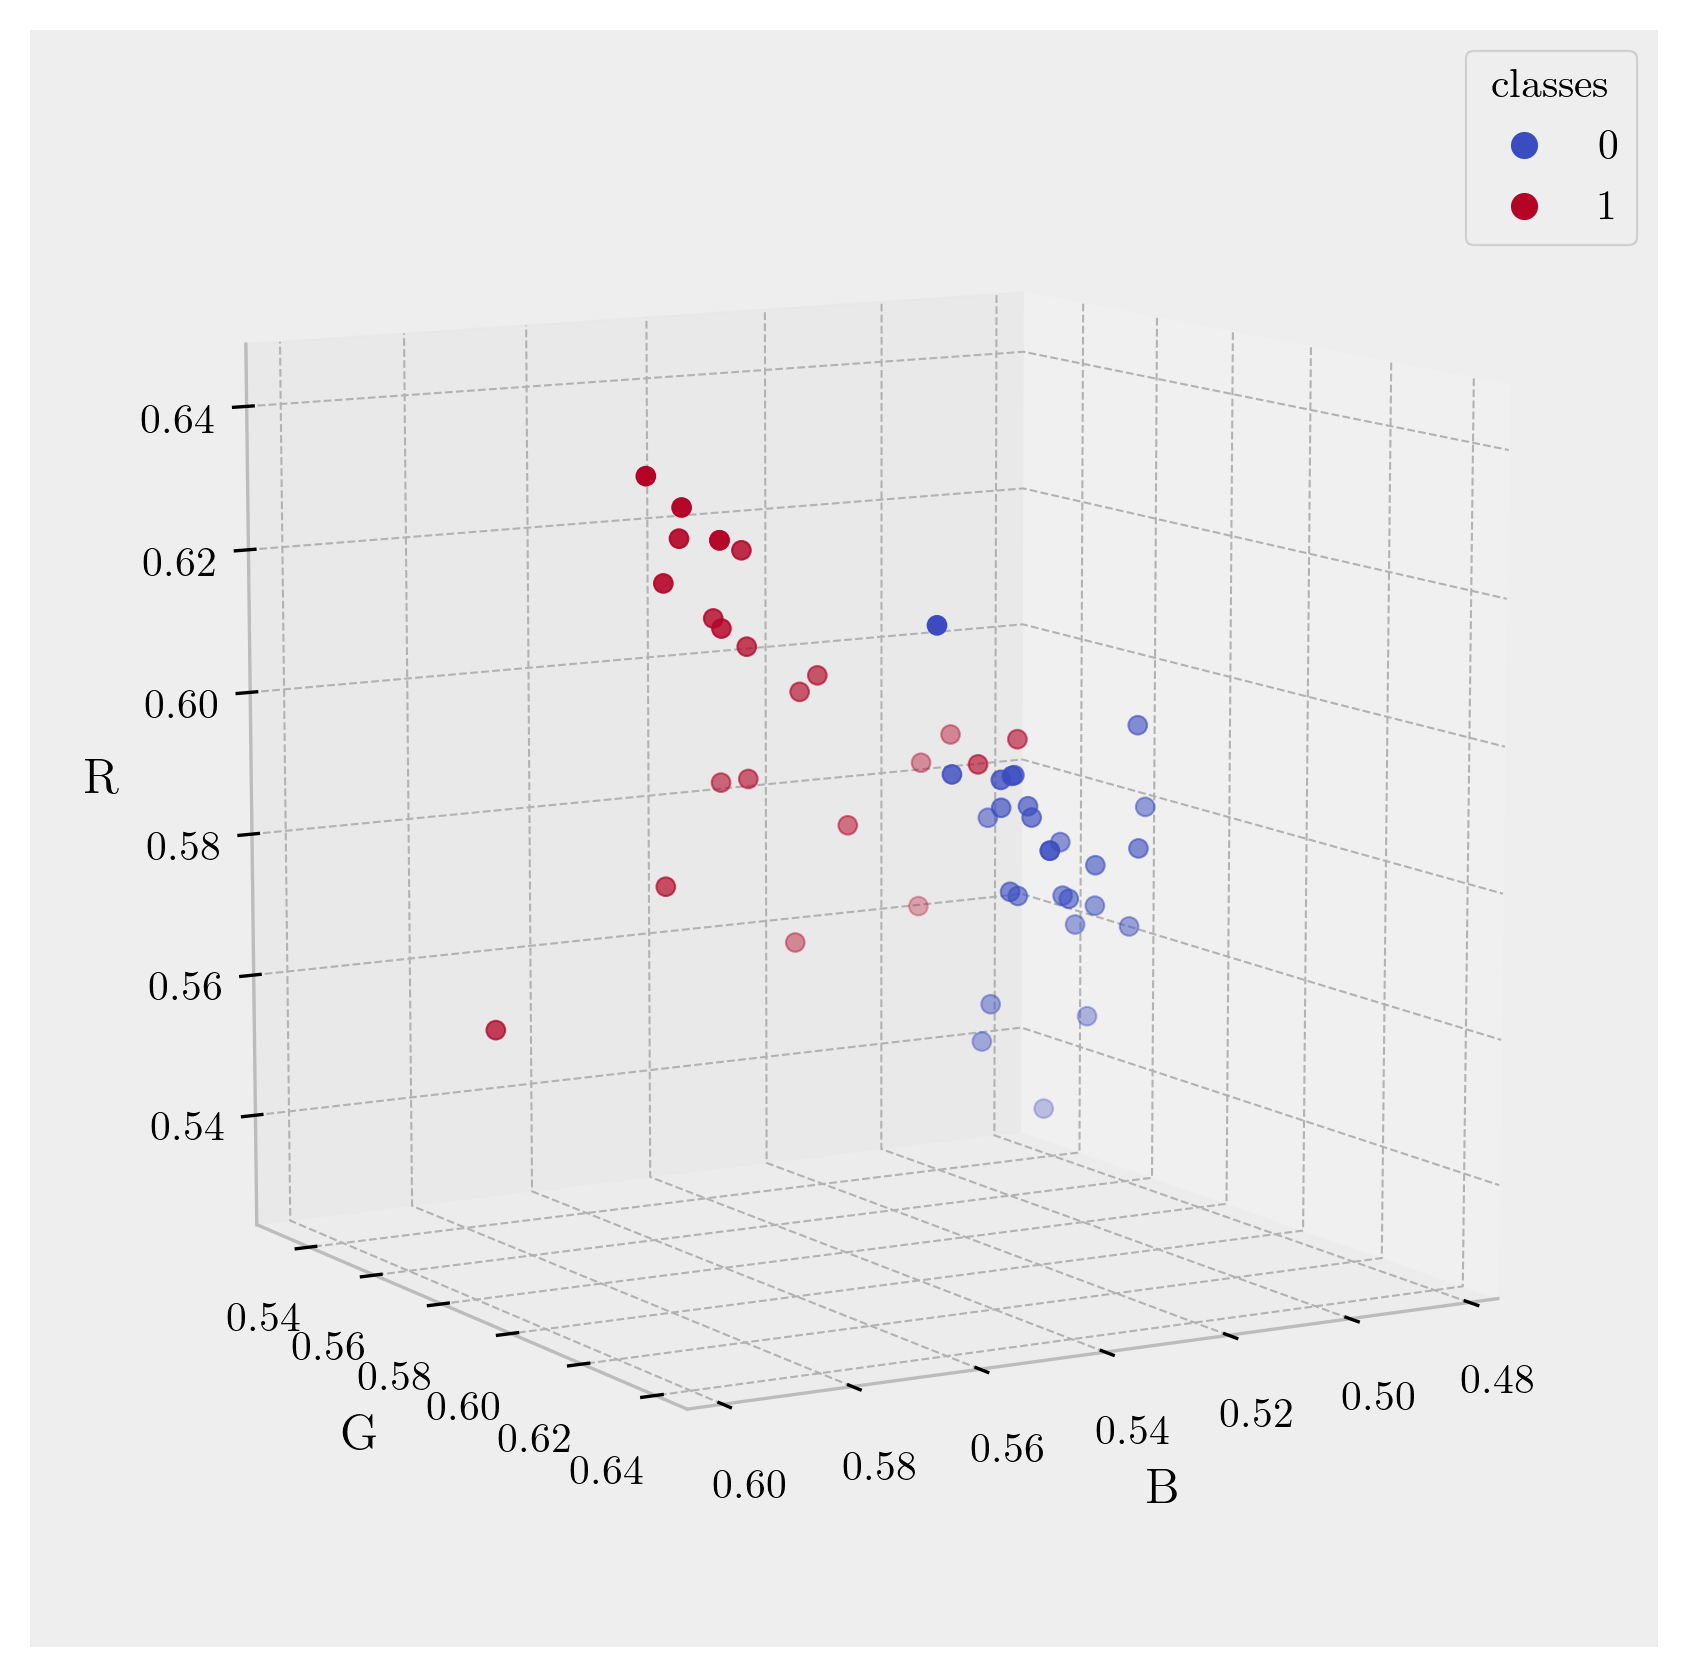
\includegraphics[width=0.8\textwidth]{RGB_extract.png}
	\caption{Feature space of ripe (1) and unripe (0) bananas in RGB.}
	\label{fig:rgb-features}
\end{figure}

\begin{figure}[htb]
	\centering
	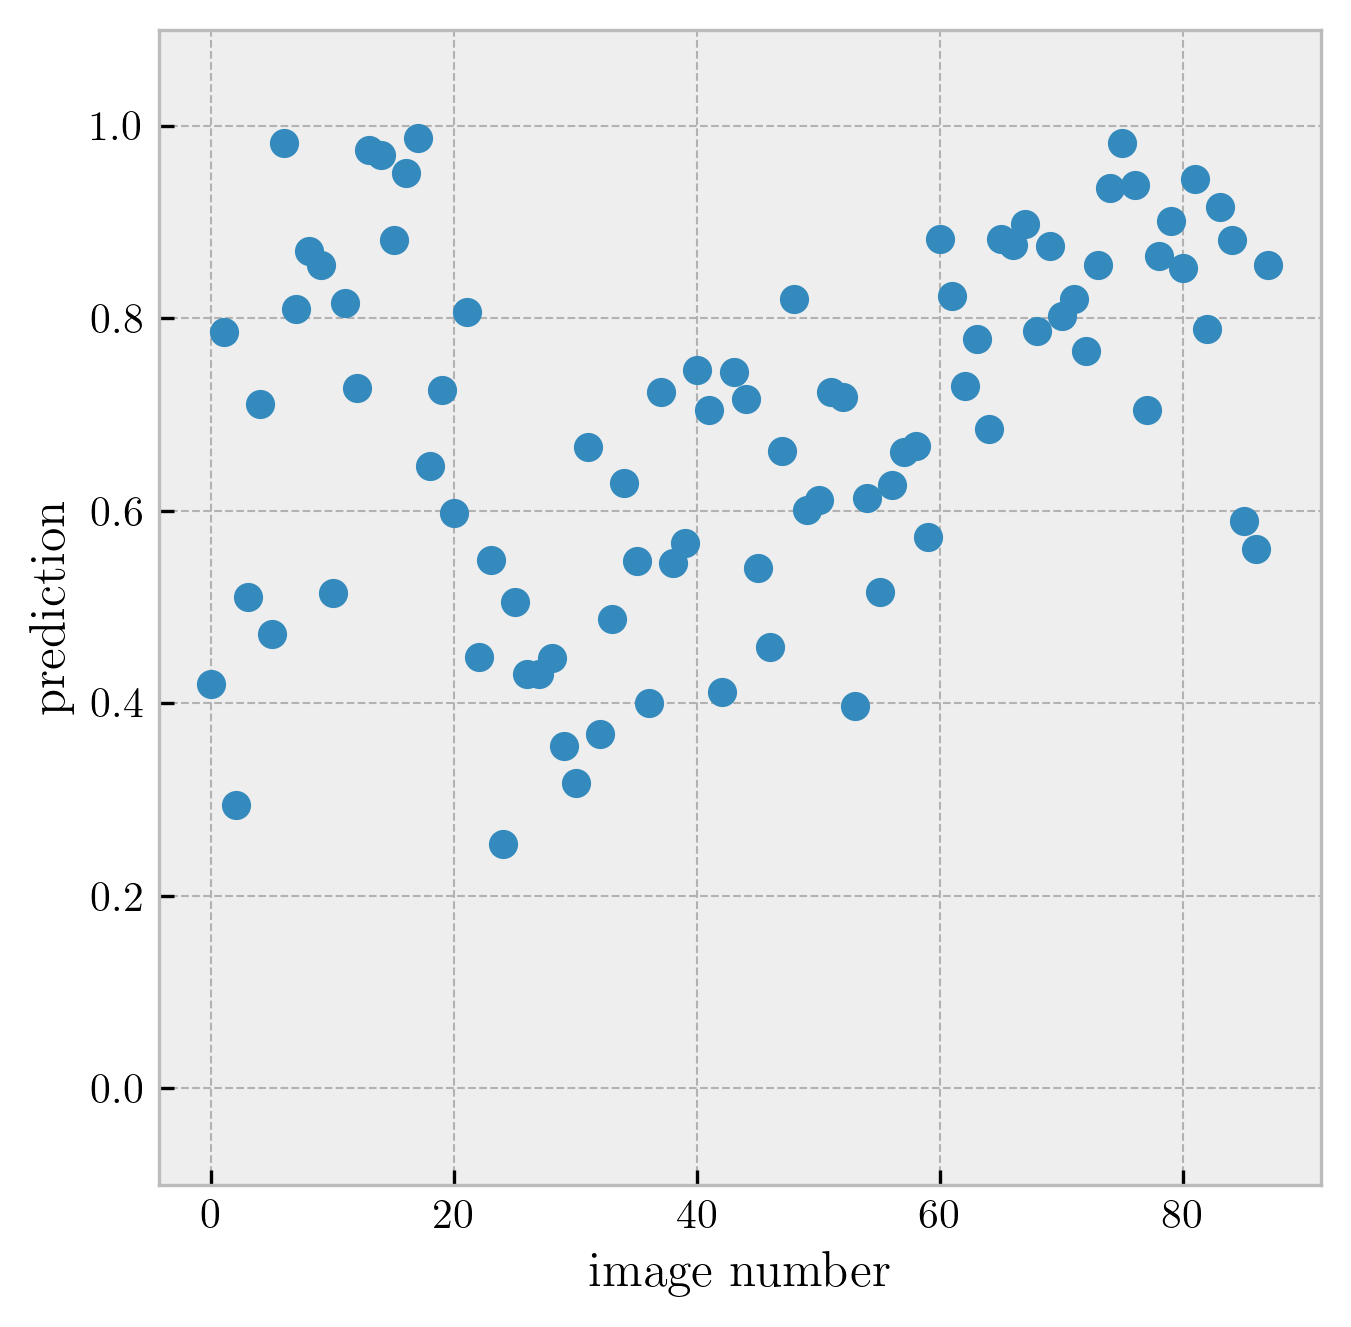
\includegraphics[width=0.5\textwidth]{RGB_preds.png}
	\caption{Final activations of the midripe banana images in RGB.}
	\label{fig:rgb-preds}
\end{figure}

\subsection{Feature extraction: $L^* a^* b^*$}
In order to be able to plot the decision contours as well as reduce the computational complexity, I decided to convert the images to $L^* a^* b^*$ color space and feed only the $a^* b^*$ features. Also, I decided to feed in overripe bananas as class 1 in order to be able to include ripe and overripe predictions. Figure \ref{fig:lab-features} shows the feature space in $L^* a^* b^*$, and we can see that the two classes are easily separable. Plotting the midripe activations in Fig. \ref{fig:lab-preds} now shows that the predictions are nicely distributed around the activation region. In Fig. \ref{fig:lab-decision}, we show the decision contours on the feature plane. In this view, we can see the sigmoid activation as a contour map---with blue being 0 and red being 1---and our training set falls in the extremes, save for a few outliers. In Fig. \ref{fig:sigmoid-map}, we show representative images for varying activation levels. We can confirm that an activation $\approx 0$ corresponds to unripe (green) bananas, an activation $\approx 1$ corresponds to overripe (yellow-brown) bananas while the regime which is approximately linear may correspond to midripe/ripe bananas. Specifically, the range $\approx$ 0.2--0.4 corresponds to the midripe (yellowish-green) bananas, while the range $\approx$ 0.6--0.8 corresponds to the ripe (dominantly yellow) bananas.

\begin{figure}[htb]
	\centering
	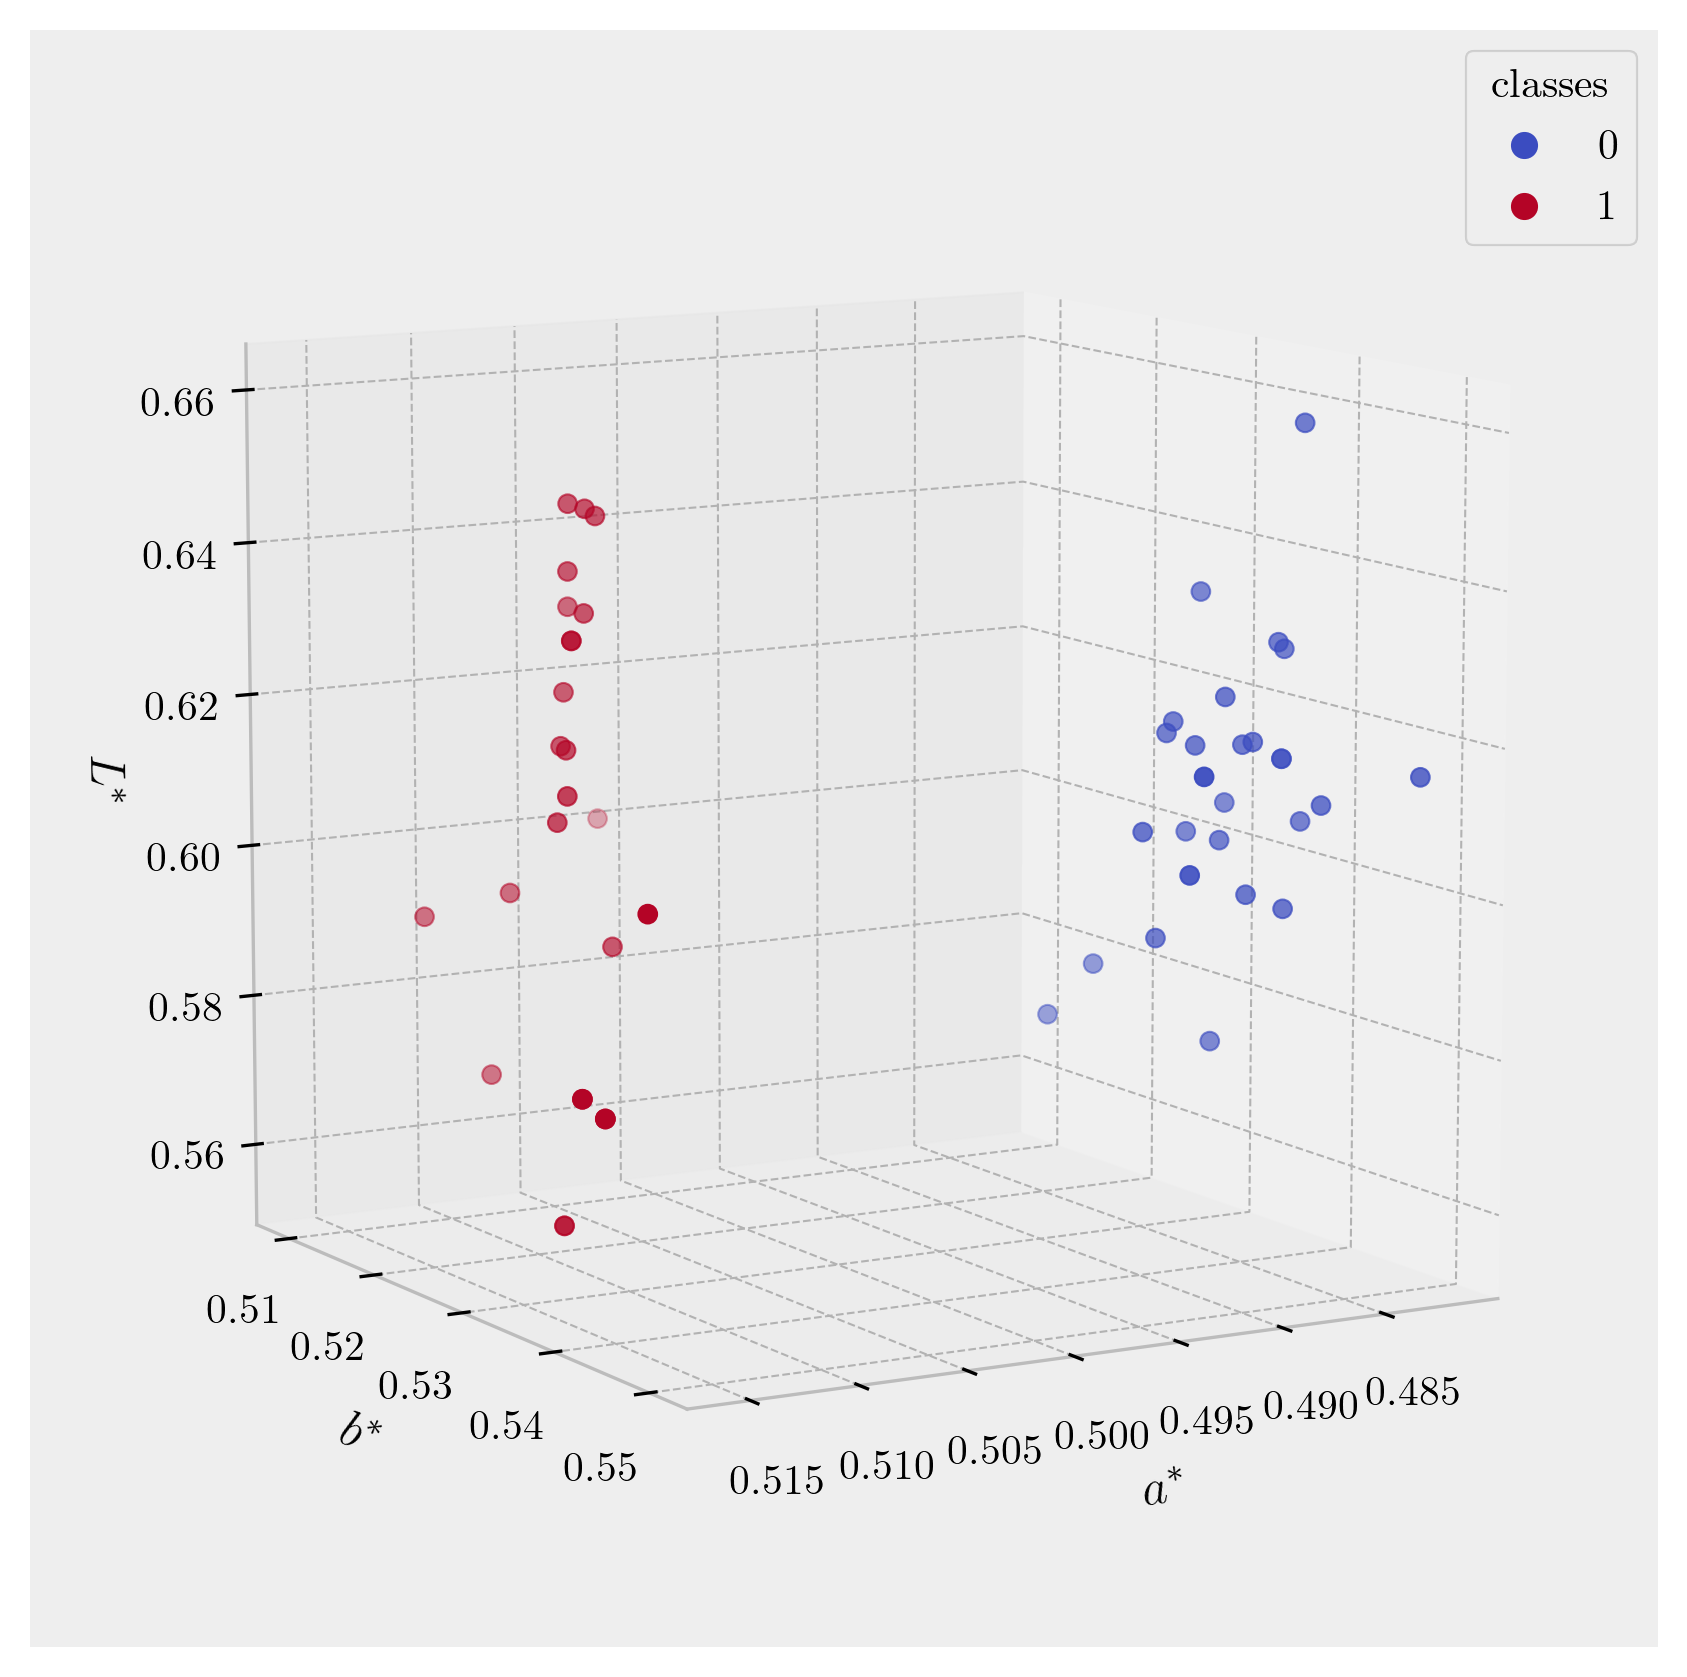
\includegraphics[width=0.8\textwidth]{Lab_extract.png}
	\caption{Feature space of overripe (1) and unripe (0) bananas in $L^* a^* b^*$.}
	\label{fig:lab-features}
\end{figure}

\begin{figure}[htb]
	\centering
	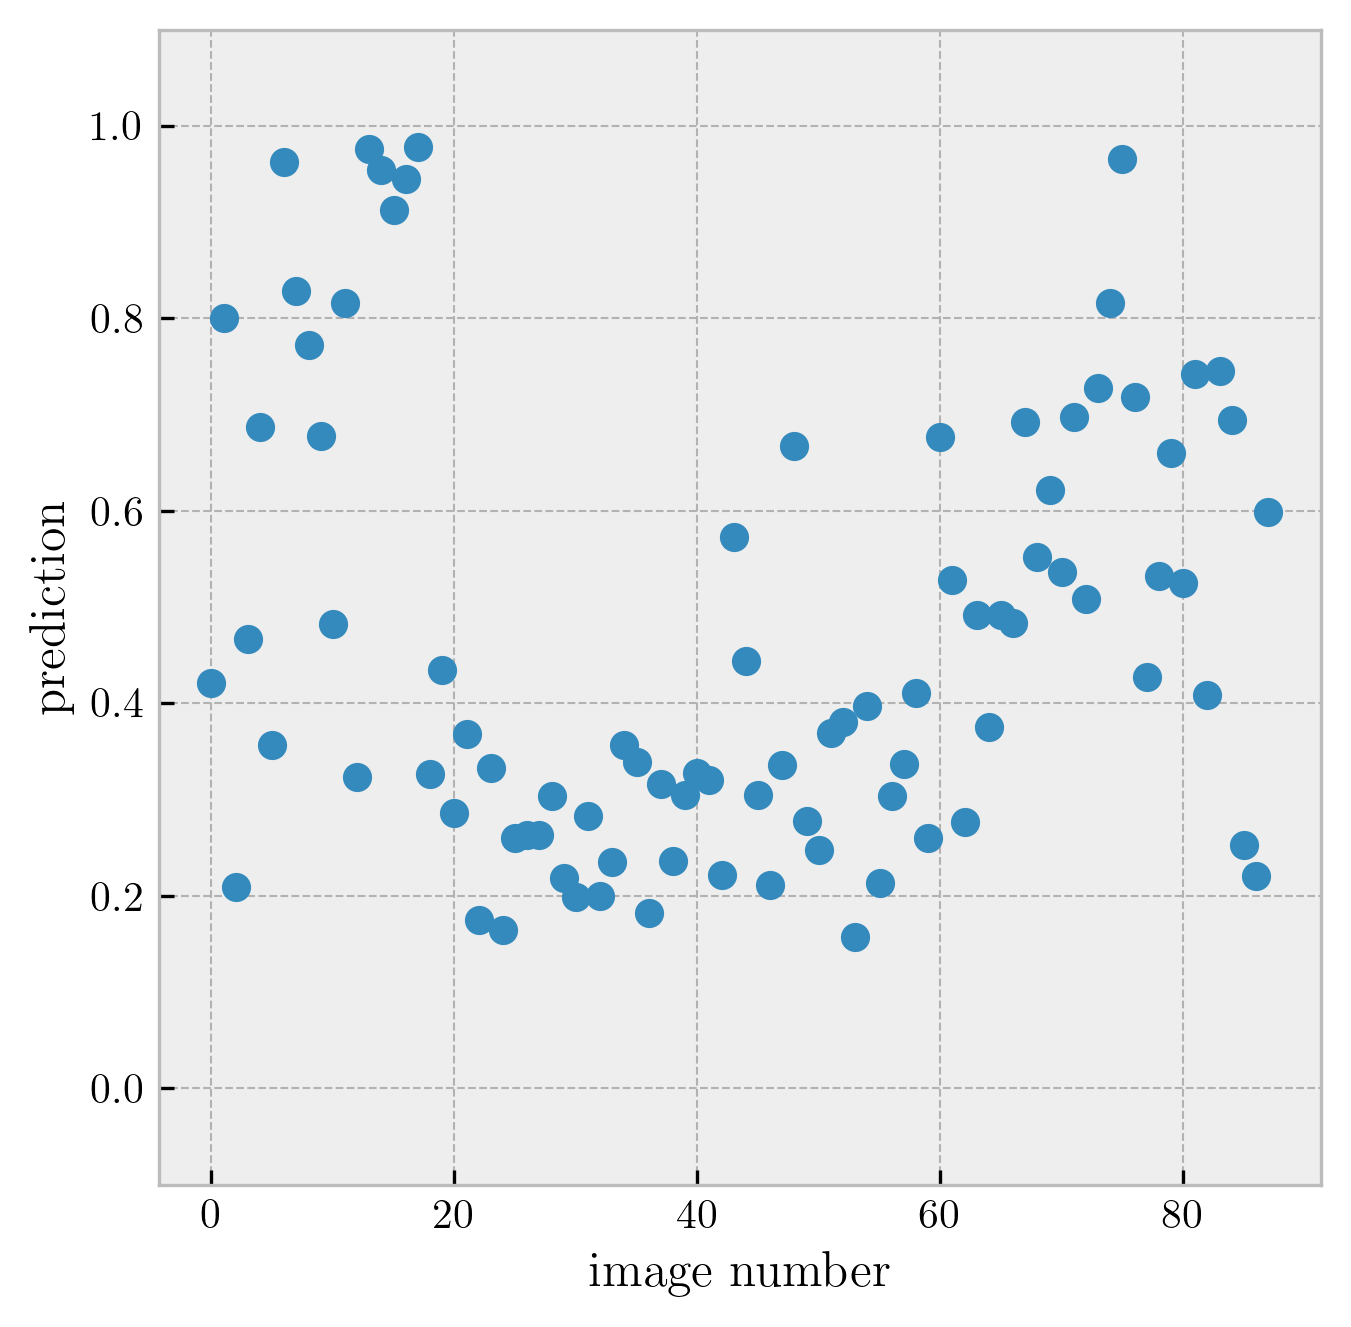
\includegraphics[width=0.5\textwidth]{Lab_preds.png}
	\caption{Final activations of the midripe banana images in $L^* a^* b^*$.}
	\label{fig:lab-preds}
\end{figure}

\begin{figure}[htb]
	\centering
	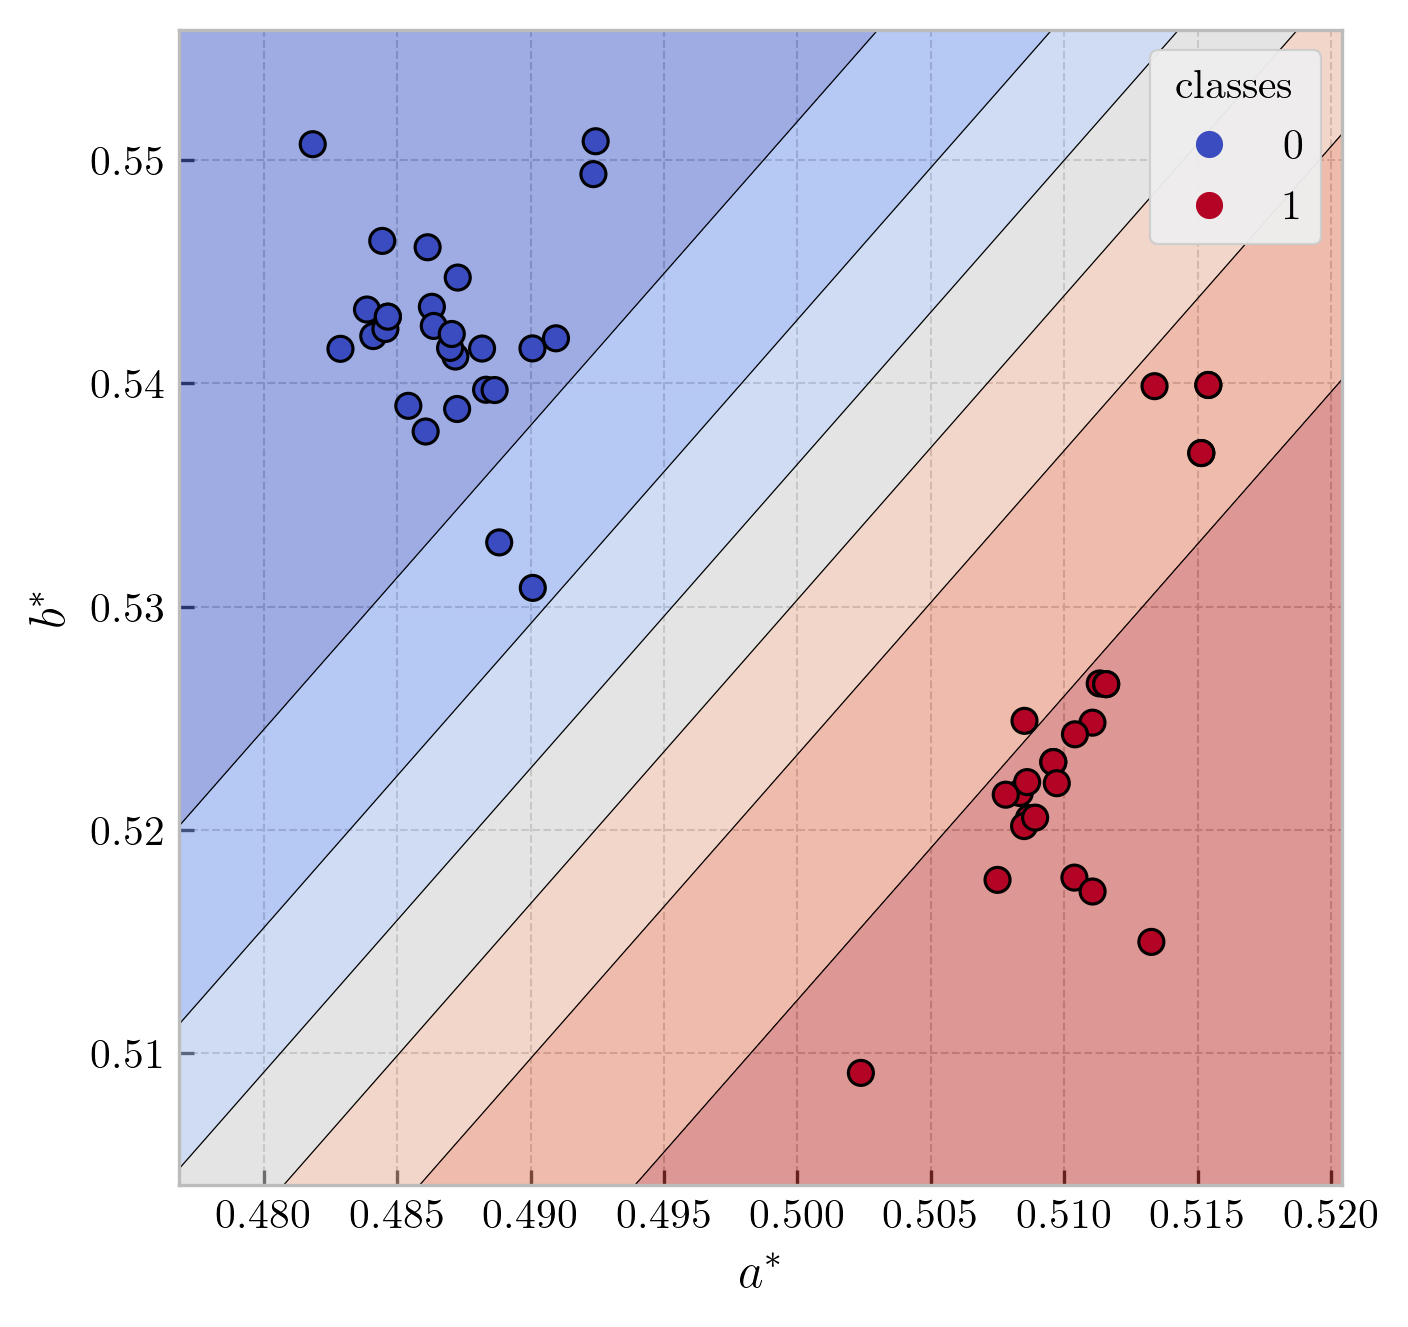
\includegraphics[width=0.7\textwidth]{Lab_decision.png}
	\caption{Decision contours of overripe (1) and unripe (0) bananas in $a^* b^*$ feature space.}
	\label{fig:lab-decision}
\end{figure}

\begin{figure}[htb]
	\centering
	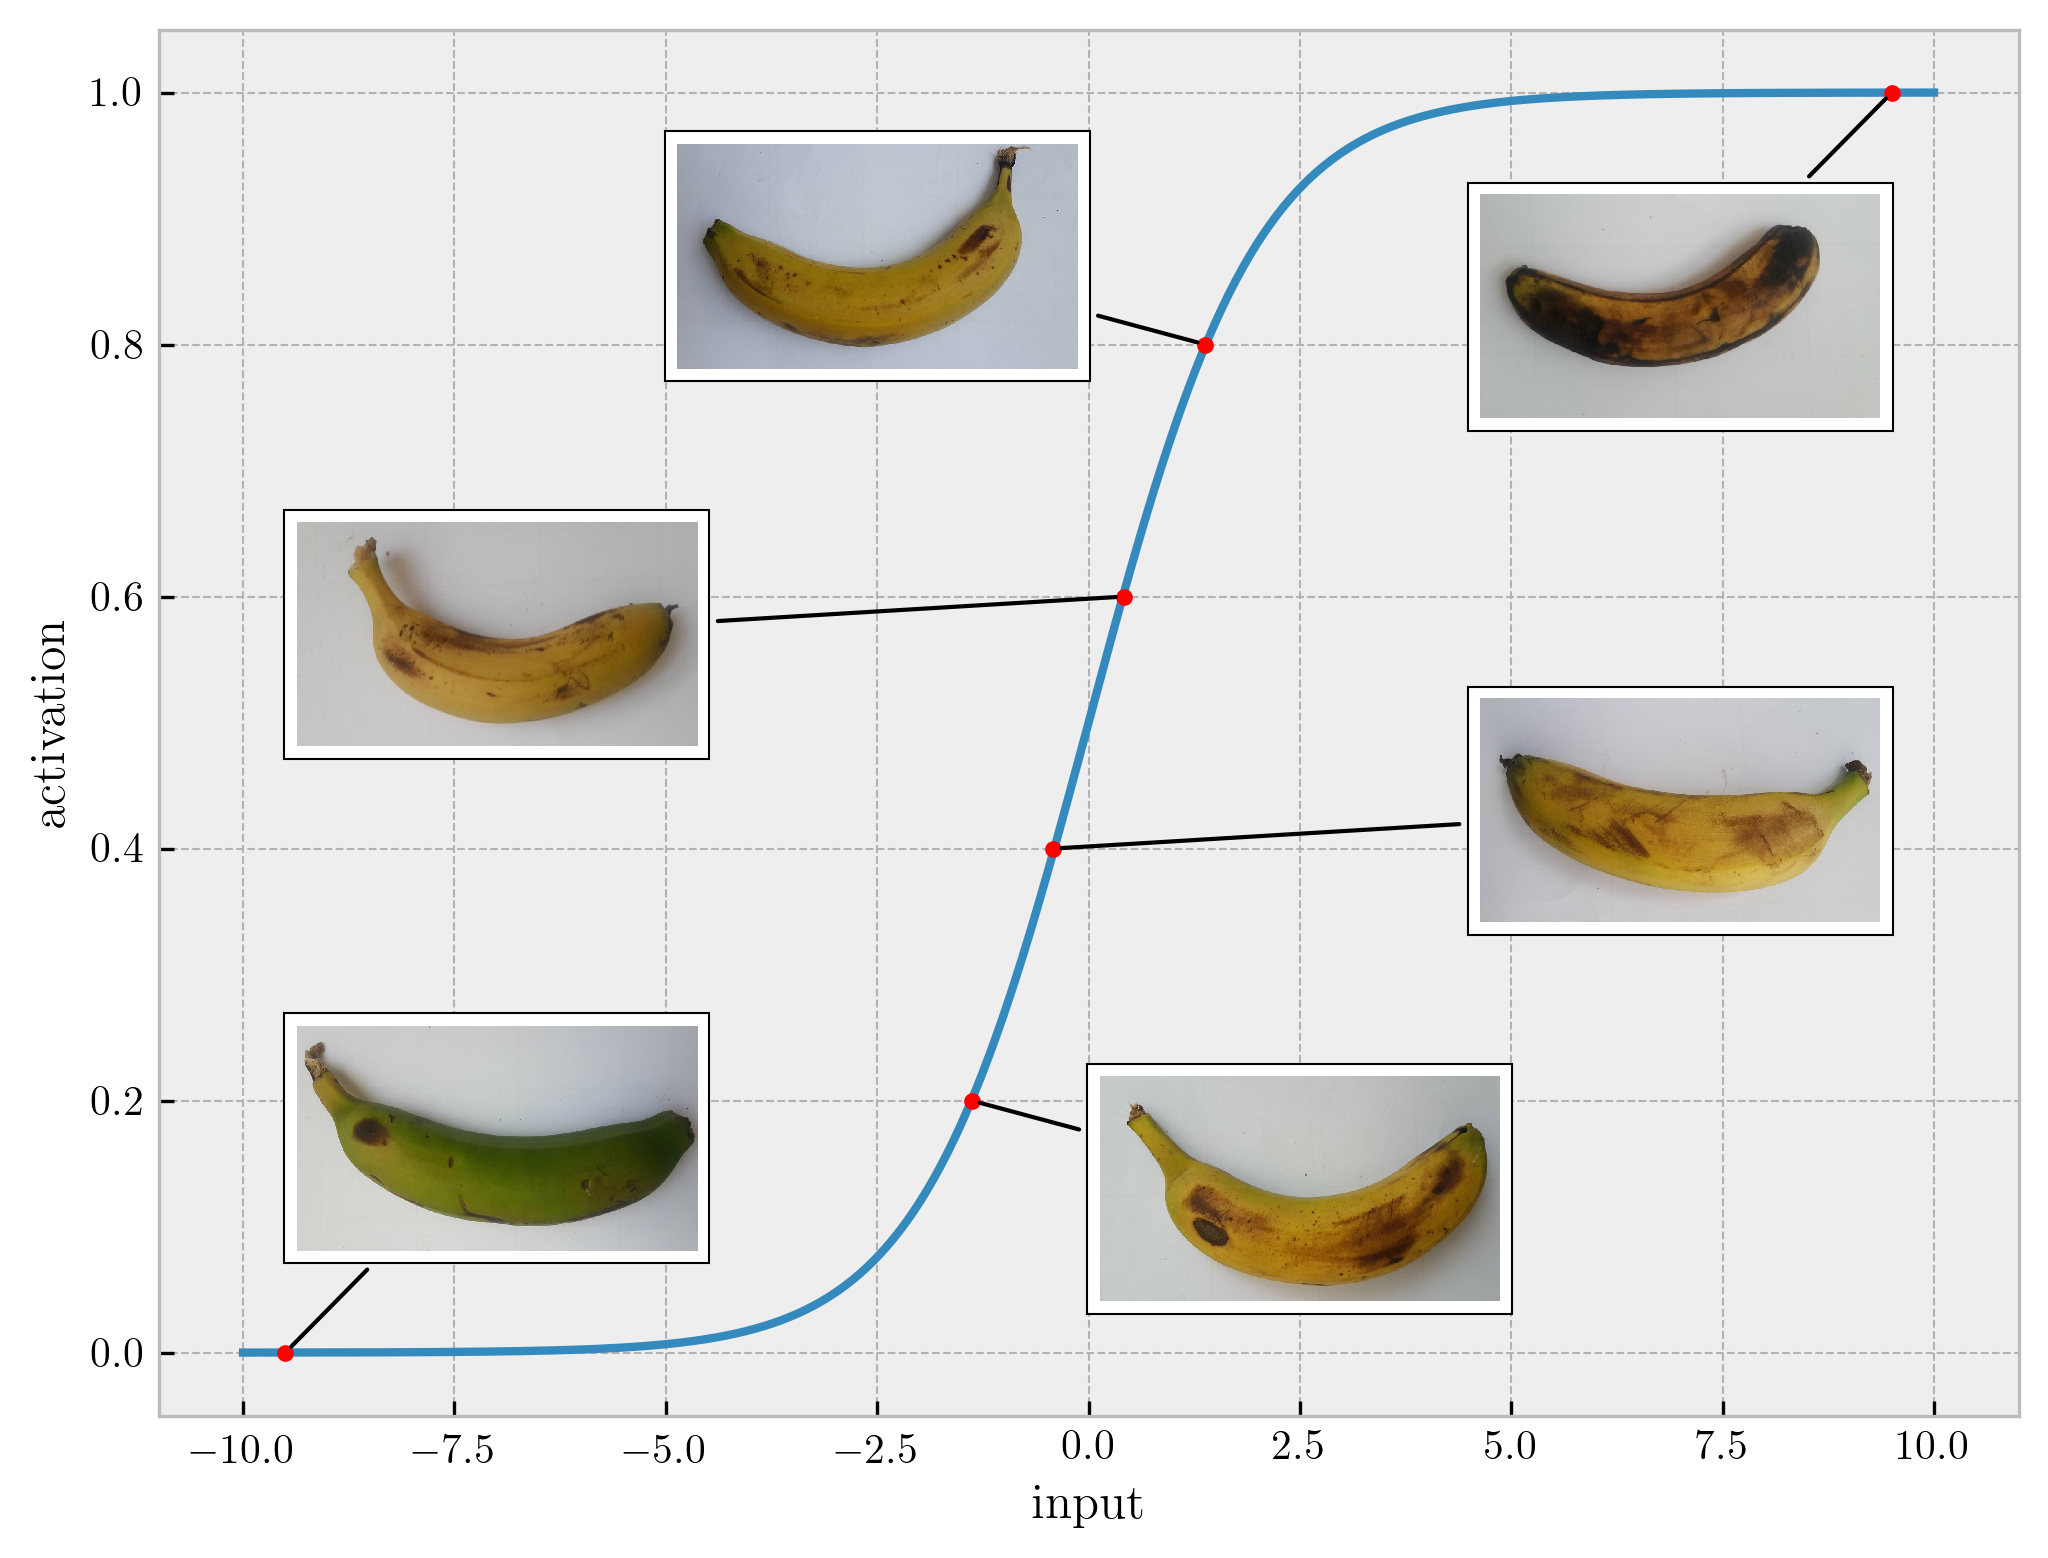
\includegraphics[width=0.8\textwidth]{sigmoid_map.png}
	\caption{Images of bananas of varying ripeness corresponding to their activation levels.}
	\label{fig:sigmoid-map}
\end{figure}


\clearpage
\begin{table}[!htb]
	\centering
	\caption{Self-evaluation.}
	\begin{tabular}{||r|c||}
		\hline
		Technical correctness & 5 \\ \hline
		Quality of presentation & 5 \\ \hline
		Initiative & 1 \\ \hline
		\textbf{TOTAL} & \textbf{11} \\ \hline
	\end{tabular}
	\label{tab:self-eval}
\end{table}

\bibliographystyle{spp-bst}
\bibliography{biblio}

\end{document}